\documentclass[11pt]{article}
\usepackage{../emch574-homework}
\homeworknumber{03}
\studentname{J.C. Vaught}
\duedate{TBD}
\begin{document}
\makehomeworktitle
\begingroup\small\sloppy\tableofcontents\endgroup
\newpage
\subsection*{Assignment}
\noindent\textbullet\quad G signifies students that take this class for Graduate Credit;\par
they must do all the items\par
\noindent\textbullet\quad UG students are not required to do the G work, but they may\par
do it for bonus points\par
\noindent\textbullet\quad Problems solved beyond the minimum requirements will be\par
given bonus points.\par
\noindent\textbullet\quad Challenge problems are optional; they will earn bonus\par
points.\par

\subsection*{NOTES}
\noindent\textbullet\quad Show your work to obtain partial credit if appropriate\par
\noindent\textbullet\quad Always display input data!\par
\noindent\textbullet\quad Partial credit might be given based on work done and\par
MATLAB codes if they are attached; without them, no partial credit can be given.\par
\noindent\textbullet\quad Display numerical results to three significant digits (four if\par
the first digit is 1).\par
\noindent\textbullet\quad Use SI system of measurement\par
https://en.wikipedia.org/wiki/International\_System\_of\_Units\par
\noindent\textbullet\quad Scale units using appropriate prefixes (e.g., nano, micro,\par
milli, kilo, mega, giga...) https://en.wikipedia.org/wiki/Metric\_prefix\par
\noindent\textbullet\quad Problems solved beyond the minimum requirements will be\par
given bonus points.\par
\noindent\textbullet\quad Challenge problems are optional. They may be solved for\par
extra credit\par
\noindent\textbullet\quad Normalized plots are plots with the y-axis scaled between\par
-1 and +1. A plotted variable is normalized by dividing it by its maximum absolute value\par
Notations and abbreviations:\par
\noindent\textbullet\quad BVP = boundary value problem\par
\noindent\textbullet\quad EOM = equation of motion\par
\noindent\textbullet\quad FBD = free body diagram\par
\noindent\textbullet\quad FRF = frequency response function\par
\noindent\textbullet\quad IVP = initial value problem\par
\noindent\textbullet\quad LHS = left hand side\par
\noindent\textbullet\quad NLM = Newton’s law of motion\par
\noindent\textbullet\quad ODE = ordinary differential equation\par
\noindent\textbullet\quad PDE = partial differential equation\par
\noindent\textbullet\quad RHS = right hand side\par
\begin{center}

\includegraphics[width=0.72\linewidth,height=0.28\textheight,keepaspectratio]{figures/extracted-000.png}
\end{center}
\section{String Vibration}
\subsection{A.1 GENERAL ANALYSIS OF STRING VIBRATION}

\begin{center}\small\itshape Figure 1 Taut string under tensile load T: (a) general view; (b)\end{center}
infinitesimal element\par

Consider a taut string of mass m per unit length stretched by a constant tension load T (Figure 1). The string undergoes small- amplitude transverse vibration with frequency ω as described by the following formula: u(x,t)=U(x)e-iωt (vibration motion) (1) Do the following:\par
\hangindent=2em\noindent\textbf{(1)} state the assumption made about the string tension T during the\par
vibration motion u\par
\hangindent=2em\noindent\textbf{(2)} draw free-body diagram (FBD) of an infinitesimal string\par
element of length ds and write sum of y forces in terms of string tension T and slope α\par
\hangindent=2em\noindent\textbf{(3)} apply small-displacement approximation and write the\par
approximate expressions for ds, sinα, sin(α+dα)\par
\hangindent=2em\noindent\textbf{(4)} write the linearized expression for the sum of y forces\par
\hangindent=2em\noindent\textbf{(5)} express the slope increment dα in terms of space increment dx\par
and the relevant partial derivative of the displacement u(x,t)\par
\hangindent=2em\noindent\textbf{(6)} apply Newton’s law of motion (NLM) and write the NLM\par
equation\par
\hangindent=2em\noindent\textbf{(7)} write the governing equation for string vibration in terms of\par
tension T, mass per unit length m, and the relevant partial derivatives of the displacement u(x,t)\par
\hangindent=2em\noindent\textbf{(8)} define wavespeed c for wave traveling in a taut string in terms\par
of tension T and mass per unit length m\par
\hangindent=2em\noindent\textbf{(9)} write the wave equation\par
\hangindent=2em\noindent\textbf{(10)} substitute Eq. (1) into item (9) and eliminate the time\par
dependency e-iωt to obtain an ODE defining U(x)\par
\hangindent=2em\noindent\textbf{(11)} recall the definition of the wavenumber γ and substitute into\par
\hangindent=2em\noindent\textbf{(10)} to obtain an ODE in terms of only γ and U(x)\par
\hangindent=2em\noindent\textbf{(12)} assume exponential solution of the form U(x)=esx\par
\hangindent=2em\noindent\textbf{(13)} develop the characteristic equation for s\par
\hangindent=2em\noindent\textbf{(14)} solve the characteristic equation and write the roots s1, s2\par
\hangindent=2em\noindent\textbf{(15)} substitute (14) into (12) and write the general solution for U(x)\par
in terms of constants A1, A2 and complex exponentials depending on γ\par
\hangindent=2em\noindent\textbf{(16)} use Euler’s formulae to rewrite (15) in terms of new constants\par
C1, C2 and trigonometric functions depending on γ\par
\hangindent=2em\noindent\textbf{(17)} substitute (16) into Eq. (1) and write the general solution for\par
u(x,t) in terms of constats C1, C2, trigonometric functions of γx and a complex exponential function of ωt\par
\hangindent=2em\noindent\textbf{(18)} Graduate Work: write the general solution for u(x,t) in terms\par
of complex exponential functions of γ and ω\par
\begin{center}
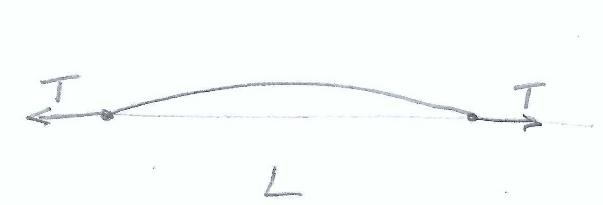
\includegraphics[width=0.72\linewidth,height=0.28\textheight,keepaspectratio]{figures/extracted-001.png}
\end{center}
\subsection{A.2 ANALYZE NATURAL FREQUENCIES AND MODESHAPES OF A}
\subsubsection*{Vibrating String}

\begin{center}\small\itshape Figure 2 Taut string of length L under constant tension T\end{center}

Consider a taut string of length L and mass m per unit length. The sting is pinned at both ends and stretched by a constant tension load T (Figure 2). The string undergoes transverse vibration with frequency ω. Do the following:\par
\hangindent=2em\noindent\textbf{(1)} write the boundary conditions at the two ends of string\par
\hangindent=2em\noindent\textbf{(2)} recall from Section A.1 the general solution for u(x,t) expressed\par
the multiplication of two terms:\par
\hangindent=2em\noindent\textbf{(a)} first term: a function U(x) depending on constants C1, C2\par
and trigonometric functions of γx\par
\hangindent=2em\noindent\textbf{(b)} second term: a complex exponential function of ωt\par
\hangindent=2em\noindent\textbf{(3)} substitute (2) into (1) and write boundary conditions in terms of\par
constants C1, C2\par
\hangindent=2em\noindent\textbf{(4)} solve (3) for C2 and obtain an equation for C1\par
\hangindent=2em\noindent\textbf{(5)} discuss the trivial solution\par
\hangindent=2em\noindent\textbf{(6)} choose to search for a nontrivial solution and define the equation\par
that needs to be solved to find a nontrivial solution\par
\hangindent=2em\noindent\textbf{(7)} introduce the notation z=γL and write the eigenvalue equation in\par
terms of z\par
\hangindent=2em\noindent\textbf{(8)} solve the eigenvalue equation and write the general expression\par
for the eigenvalues zj , j=1,2,3,...\par
\hangindent=2em\noindent\textbf{(9)} use (8) to write the general expression for the wavenumber γj in\par
terms of j and length L\par
\hangindent=2em\noindent\textbf{(10)} Recall from HW01 the definition of wavenumber γ in terms of\par
frequency ω and wavespeed c\par
\hangindent=2em\noindent\textbf{(11)} solve (10) for frequency ω in terms of wavenumber γ and\par
wavespeed c\par
\hangindent=2em\noindent\textbf{(12)} use (9) and (11) to write the general expression of the natural\par
frequency ωj in terms of j, wavespeed c, and string length L\par
\hangindent=2em\noindent\textbf{(13)} use (12) to write the general expression of the Hz frequency fj\par
in terms of j, wavespeed c, and string length L\par
\hangindent=2em\noindent\textbf{(14)} explain the meaning of fundamental frequency and overtones\par
\hangindent=2em\noindent\textbf{(15)} recall from HW01 the relationship between wavelength λ and\par
wavenumber γ\par
\hangindent=2em\noindent\textbf{(16)} use (9) into (15) to write the general expression for the\par
wavelength λj in terms of j and string length L\par
\hangindent=2em\noindent\textbf{(17)} use (16) to explain which wavelength multiples could\par
accommodate vibratory standing waves in a string of length L fixed at both ends\par
\hangindent=2em\noindent\textbf{(18)} recall from (2)(a) the expression for U(x)\par
\hangindent=2em\noindent\textbf{(19)} use (4) to eliminate C2\par
\hangindent=2em\noindent\textbf{(20)} set C1=1 in (19) and write the general expression of the\par
modeshape Uj(x) in terms of the wavenumber γj\par
\hangindent=2em\noindent\textbf{(21)} give the expression of modeshape orthonormality\par
\subsection{A.3 CALCULATE STRING VIBRATION}
Consider a taught string of length L=22 inches tuned to the note G3. The purpose is to calculate the string vibration characteristics and the modeshapes for j=1,...,N modes with N=5. We should also verify mode orthonormality using numerical integration on a linspace(0,L,Nx) with Nx=1000. Recall the appropriate results from in-class instruction class and BB notes to do the following:\par
\hangindent=2em\noindent\textbf{(1)} Display input data\par
\hangindent=2em\noindent\textbf{(2)} State the note symbol (letter and octave) and the corresponding\par
fundamental Hz frequency f1 of the string.\par
\hangindent=2em\noindent\textbf{(3)} Use frequency f1 and length L to calculate the wavespeed c\par
\hangindent=2em\noindent\textbf{(4)} Calculate and display modal wavenumbers γj and frequencies ωj\par
\hangindent=2em\noindent\textbf{(5)} Calculate the modeshapes, plot each mode separately and then\par
plot overlapped all the N modes in a single plot\par
\hangindent=2em\noindent\textbf{(6)} Verify modeshape orthonormality by numerical integration\par
\hangindent=2em\noindent\textbf{(7)} Discuss your results\par
\begin{center}
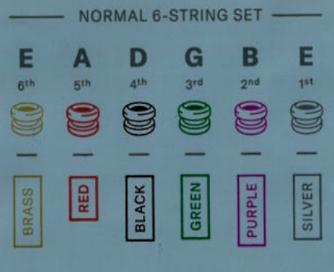
\includegraphics[width=0.72\linewidth,height=0.28\textheight,keepaspectratio]{figures/extracted-002.png}
\end{center}
\subsection{A.4 CALCULATE D’ADDARIO GUITAR STRINGS}

\begin{center}\small\itshape Table 1\end{center}
\subsubsection*{Brass Red Black Green Purple Silver}
musical\par
\subsubsection*{E A D G B E}
note M, grams 6.42 4.18 2.45 1.332 0.655 0.367 T, lbf 24.95 28.93 29.93 30.05 23.31 23.36\par

Consider a set of six light-gauge d’Addario guitar strings. All six strings have the same length L=25.0 inches. The mass M and the tension T of each string are given in in Table 1.\par
\hangindent=2em\noindent\textbf{(1)} Display input data\par
For each of the six strings, do the following:\par
\hangindent=2em\noindent\textbf{(2)} Display string length L in m\par
\hangindent=2em\noindent\textbf{(3)} Calculate and display distributed mass, m, in kg/m\par
\hangindent=2em\noindent\textbf{(4)} Display tension T in N\par
\hangindent=2em\noindent\textbf{(5)} Calculate wavespeed c in m/s\par
\hangindent=2em\noindent\textbf{(6)} Calculate fundamental frequency f1 in Hz\par
\hangindent=2em\noindent\textbf{(7)} Find the musical note that most closely approximates the\par
frequency and give its letter name and octave number (e.g., G3 signifies note G in the 3rd octave)\par
\hangindent=2em\noindent\textbf{(8)} Display the frequency of the musical notes found at (7)\par
\hangindent=2em\noindent\textbf{(9)} Calculate the percentage difference between your findings and\par
the nominal frequency of that musical note\par
\hangindent=2em\noindent\textbf{(10)} Comment on your findings and identify possible sources of\par
error.\par
\hangindent=2em\noindent\textbf{(11)} Graduate work: Calculate the necessary adjustments in mass,\par
tension, or both to achieve frequency match within 0.00\%\par
\begin{center}
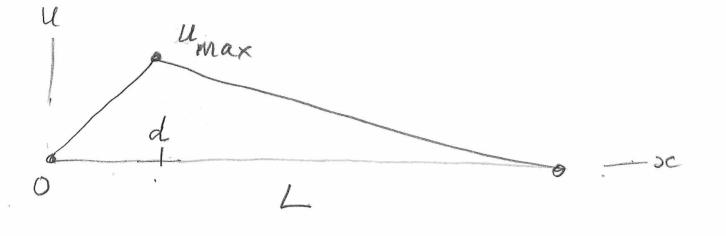
\includegraphics[width=0.72\linewidth,height=0.28\textheight,keepaspectratio]{figures/extracted-003.png}
\end{center}
\subsection{A.5 CALCULATE VIBRATION OF A PLUCKED STRING}

\begin{center}\small\itshape Figure 3 Taut string plucked at an arbitrary location d\end{center}

Consider a taught string of length L=25.5 inches tuned to the note G3. The string is plucked by applying an initial displacement umax=1.25mm at a location d. In this problem, we will consider three possible plucking locations: d=L/2, L/4, 7L/10. The purpose is to calculate the response u(x,t) of the plucked string using the modal expansion method with N=10. Recall the appropriate results from in-class instruction class and BB notes to do the following:\par
\hangindent=2em\noindent\textbf{(1)} Display input data\par
\hangindent=2em\noindent\textbf{(2)} State the note symbol (letter and octave) and the corresponding\par
fundamental Hz frequency f1 of the string. Calculate the corresponding fundamental mode period τ1.\par
\hangindent=2em\noindent\textbf{(3)} Use frequency f1 and length L to calculate the wavespeed c\par
\hangindent=2em\noindent\textbf{(4)} Calculate modal wavenumbers γj and frequencies ωj\par
\hangindent=2em\noindent\textbf{(5)} Calculate and plot overlapped the N modes\par
\hangindent=2em\noindent\textbf{(6)} For each plucking location, do the following:\par
\hangindent=2em\noindent\textbf{(a)} display the value d and plot the initial shape of the string\par
u0(x)\par
\hangindent=2em\noindent\textbf{(b)} calculate by numerical integration the modal participation\par
factors Aj, display Aj in mm, and do a bar plot\par
\hangindent=2em\noindent\textbf{(c)} plot the time response of the string at the plucking location\par
u(d,t) for t=0,...,tmax with tmax=3τ1\par
\hangindent=2em\noindent\textbf{(d)} Graduate work: reconstruct the initial string shape and\par
plot it overlapped on the actual shape\par
\hangindent=2em\noindent\textbf{(7)} Discuss comparatively the results for the three plucking\par
locations\par
\begin{center}
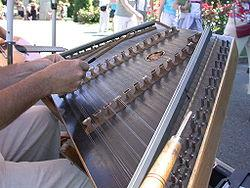
\includegraphics[width=0.72\linewidth,height=0.28\textheight,keepaspectratio]{figures/extracted-004.png}
\end{center}
\begin{center}

\includegraphics[width=0.72\linewidth,height=0.28\textheight,keepaspectratio]{figures/extracted-005.png}
\end{center}
\subsection{A.6 CALCULATE FREQUENCY RESPONSE OF A STRUCK STRING}
This problem addresses the frequency response of a taut string when struck by a point load like in the case of the hammered dulcimer (Figure 4).\par

\hangindent=2em\noindent\textbf{(a)} \par

\hangindent=2em\noindent\textbf{(b)} \par
\begin{center}\small\itshape Figure 4 Struck string: (a) the hammered dulcimer; (b) schematic\end{center}

Consider a taught string of length L=25.5 inches and distributed mass m=0.0015 kg/m tuned to the note G3. The string damping ratio is assumed to have same value ζ0=2.1\% in all modes. The string is struck at location xe. The response of the string is measured with a piezoelectric acoustic pickup at location x0. Three xe, x0 cases are considered: case xe x0\par
\hangindent=2em\noindent\textbf{(a)} L/3 L/3\par
\hangindent=2em\noindent\textbf{(b)} L/3 L/2\par
\hangindent=2em\noindent\textbf{(c)} L/2 L/2\par
The striking force is assumed harmonic with amplitude Fe=0.5 N and frequency range fstart=20 Hz through fend=2000 Hz with Nf=5000 steps. The objective is to calculate and plot the frequency response\par
function (FRF) over the frequency range using modal expansion method with N=10 modes. Do the following:\par
\hangindent=2em\noindent\textbf{(1)} Display input data\par
\hangindent=2em\noindent\textbf{(2)} State the note name and octave and the corresponding\par
fundamental Hz frequency f1 of the string. Calculate the corresponding period τ1 and the wavespeed c\par
\hangindent=2em\noindent\textbf{(3)} For j=1,...,N, calculate and display the modal properties\par
wavenumber γj, frequency ωj, mass mj; damping ζj and plot overlapped the modeshapes\par
\hangindent=2em\noindent\textbf{(4)} Define the frequency range f using linspace(fstart, fend, Nf) and\par
then define ω=2πf\par
\hangindent=2em\noindent\textbf{(5)} For each xe,x0 case, plot the |FRF(ω ; xe,x0)| in dB and find the\par
frequencies and nearest musical notes, as well as the index of the string modal frequency\par
\hangindent=2em\noindent\textbf{(6)} Graduate work: plot the time response of the normalized sound\par
picked up at x0=L/2 when the string was struck at xe=L/3. The excitation frequency should be the dominant note frequency in the FRF plot. The time plot should cover three periods of the dominant frequency.\par
\begin{center}
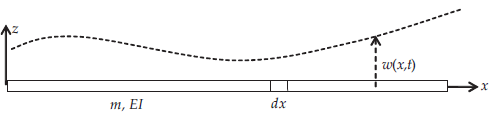
\includegraphics[width=0.72\linewidth,height=0.28\textheight,keepaspectratio]{figures/extracted-006.png}
\end{center}
\section{Flexural Vibration}
\subsection{B.1 GENERAL ANALYSIS OF FLEXURAL VIBRATION}
Consider a uniform beam of mass m per unit length and bending stiffness EI undergoing flexural motion with vertical displacement w(x,t) as shown in Figure 5. Centroidal axes are assumed.\par

\begin{center}\small\itshape Figure 5 Beam undergoing flexural vibration\end{center}

Do the following:\par
\hangindent=2em\noindent\textbf{(1)} state the assumptions needed for performing the flexural\par
vibration analysis\par
\hangindent=2em\noindent\textbf{(2)} draw free-body diagram (FBD) of an infinitesimal beam\par
element dx and show the stress resultants N, M, V.\par
\hangindent=2em\noindent\textbf{(3)} write the definitions of the stress resultants N and M\par
\hangindent=2em\noindent\textbf{(4)} use stress-strain relation to write the stress resultants in terms\par
of strains\par
\hangindent=2em\noindent\textbf{(5)} perform kinematic analysis to express the stress resultant M in\par
terms of partial derivatives of the displacement w\par
\hangindent=2em\noindent\textbf{(6)} perform free-body analysis of the infinitesimal element dx and\par
find the sum of forces ΣFz and sum of moments ΣM\par
\hangindent=2em\noindent\textbf{(7)} apply Newton’s law of motion (NLM) in the z direction and\par
obtain an equation for the shear force V\par
\hangindent=2em\noindent\textbf{(8)} apply NLM in the rotational direction and obtain an equation\par
for the moment M\par
\hangindent=2em\noindent\textbf{(9)} substitute (6) into (8) and get an equation that relates M and V\par
\hangindent=2em\noindent\textbf{(10)} use (5) into (9) and obtain the governing equation\par
\hangindent=2em\noindent\textbf{(11)} define the flexural constant a in terms of E, I, m\par
\hangindent=2em\noindent\textbf{(12)} use (11) into (10) to obtain the governing equation as a PDE in\par
x, t, and flexural constant a\par
\hangindent=2em\noindent\textbf{(13)} assume harmonic vibration of the form w(x,t)=W(x)e-iωt\par
\hangindent=2em\noindent\textbf{(14)} substitute (13) into (12) and obtain an ODE in x with constants\par
a, ω\par
\hangindent=2em\noindent\textbf{(15)} define the wavenumber γ in terms of ω and a and substitute in\par
\hangindent=2em\noindent\textbf{(14)} to write the ODE with only one constant, γ\par
\hangindent=2em\noindent\textbf{(16)} assume W(x) as an exponential function of x of the form =esx\par
\hangindent=2em\noindent\textbf{(17)} substitute (16) into (15) and derive the characteristic equation\par
\hangindent=2em\noindent\textbf{(18)} find the four roots of the characteristic equation\par
\hangindent=2em\noindent\textbf{(19)} write the general solution W(x) in terms of constants A1, A2,\par
A3, A4 and complex exponential functions of γx\par
\hangindent=2em\noindent\textbf{(20)} rewrite the general solution (19)(13) in terms of constats C1, C2,\par
C3, C4 multiplying trigonometric and hyperbolic functions of γx\par
\hangindent=2em\noindent\textbf{(21)} Graduate Work: explain how one can find the constants C1,\par
\subsubsection*{C2, C3, C4}
\begin{center}
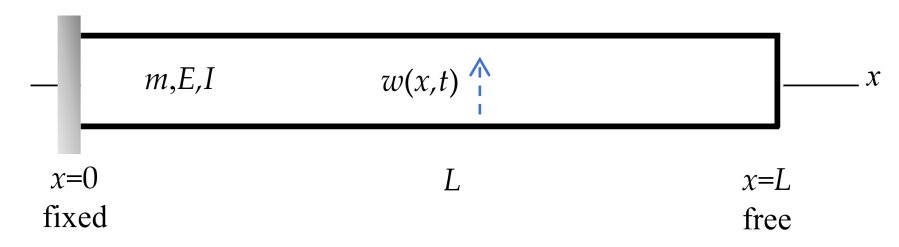
\includegraphics[width=0.72\linewidth,height=0.28\textheight,keepaspectratio]{figures/extracted-007.png}
\end{center}
\subsection{B.2 ANALYZE CANTILEVER BEAM VIBRATION}
A cantilever beam is fixed at one end and free at the other end. Consider a cantilever beam of length L as shown in Figure 6. The beam has mass density per unit length m, elastic modulus E, and cross-section second moment of area I.\par

\begin{center}\small\itshape Figure 6 Vibration of a cantilever beam of length L. The cantilever\end{center}
beam is fixed at one end and free at the other end\par

Do the following:\par
\hangindent=2em\noindent\textbf{(1)} write the boundary conditions at the two ends of the bar\par
\hangindent=2em\noindent\textbf{(2)} recall from the notes the general solution w(x,t) consisting of\par
the multiplication of two terms:\par
\hangindent=2em\noindent\textbf{(a)} first term: a function W(x) depending on constants C1, C2,\par
C3, C4, and trigonometric and hyperbolic functions of γx\par
\hangindent=2em\noindent\textbf{(b)} second term: a complex exponential function of ωt\par
\hangindent=2em\noindent\textbf{(3)} substitute (2) into (1) and write boundary conditions in terms\par
of constants C1, C2, C3, C4\par
\hangindent=2em\noindent\textbf{(4)} solve (3) for C3, C4 in terms of C1, C2 and obtain a set of\par
equations for C1, C2\par
\hangindent=2em\noindent\textbf{(5)} discuss the trivial solution\par
\hangindent=2em\noindent\textbf{(6)} choose to search for a nontrivial solution and define the\par
equation that needs to be solved to find a nontrivial solution\par
\hangindent=2em\noindent\textbf{(7)} introduce the notation z=γL and write the transcendental\par
eigenvalue equation in terms of z\par
\hangindent=2em\noindent\textbf{(8)} use the MATLAB function fzero to solve the transcendental\par
eigenvalue equation and find zj, j=1,...,N with N=5\par
\hangindent=2em\noindent\textbf{(9)} use item (7) to write the general expression for the\par
wavenumber γj in terms of zj and length L\par
\hangindent=2em\noindent\textbf{(10)} Recall from Problem B.1 the definition of wavenumber γ in\par
terms of frequency ω and flexural constant a\par
\hangindent=2em\noindent\textbf{(11)} solve (10) for frequency ω in terms of wavenumber γ and\par
flexural constant a\par
\hangindent=2em\noindent\textbf{(12)} use (9) and (11) to write the general expression of the natural\par
frequency ωj in terms of eigenvalue zj, beam constant a, and beam length L\par
\hangindent=2em\noindent\textbf{(13)} recall definition of a in terms of bending stiffness EI and mass\par
per unit length m and obtain an expression for the natural frequencies ωj and fj in terms of zj, EI, m, L\par
\hangindent=2em\noindent\textbf{(14)} use (4) to obtain an expression for the ratio C1/C2 in terms of\par
wavenumber γ and beam length L. Denote this expression to be -β\par
\hangindent=2em\noindent\textbf{(15)} recall from (2)(a) the expression for W(x)\par
\hangindent=2em\noindent\textbf{(16)} use (4) and (14) to write the constants C1, C3, C4 in terms of\par
C2\par
\hangindent=2em\noindent\textbf{(17)} substitute (16) into (15) and write W(x) in terms of C2, γx, β\par
\hangindent=2em\noindent\textbf{(18)} Set C2=1 and write the modeshapes Wj(x) in terms of γj and\par
βj\par
\hangindent=2em\noindent\textbf{(19)} give the expression of modeshape orthonormality\par
\hangindent=2em\noindent\textbf{(20)} Graduate work:\par
\hangindent=2em\noindent\textbf{(a)} write the approximate expression for the eigenvalues zj\par
with j>=6\par
\hangindent=2em\noindent\textbf{(b)} solve the transcendental equation at item (7) for N=10 and\par
compare with the prediction using the approximate expression of item (a)\par
\subsection{B.3 CALCULATE CANTILEVER BEAM VIBRATION}
Assume a cantilever beam of length L=445mm and cross-section dimensions h=3mm, b=37mm. The material is steel with E=200GPa and ρ=7850 kg/m3. Do the following:\par
\hangindent=2em\noindent\textbf{(1)} display input data\par
\hangindent=2em\noindent\textbf{(2)} calculate the cross-section area A\par
\hangindent=2em\noindent\textbf{(3)} calculate mass per unit length m\par
\hangindent=2em\noindent\textbf{(4)} calculate second moment of area I\par
\hangindent=2em\noindent\textbf{(5)} calculate flexural stiffness EI\par
\hangindent=2em\noindent\textbf{(6)} calculate flexural constant a\par
\hangindent=2em\noindent\textbf{(7)} solve the transcendental equation defined in Problem B.2\par
item (7) to find zj, j=1,...,N with N=5\par
\hangindent=2em\noindent\textbf{(8)} calculate the wavenumbers γj\par
\hangindent=2em\noindent\textbf{(9)} calculate angular frequencies ωj\par
\hangindent=2em\noindent\textbf{(10)} calculate Hz frequencies fj\par
\hangindent=2em\noindent\textbf{(11)} calculate the modeshape coefficients βj\par
\hangindent=2em\noindent\textbf{(12)} calculate the modeshapes Wj(x), plot each mode separately\par
and then plot overlapped all the N modes on a single plot\par
\hangindent=2em\noindent\textbf{(13)} verify modeshape orthonormality by numerical integration\par
\hangindent=2em\noindent\textbf{(14)} comment on your results\par
\begin{center}

\includegraphics[width=0.72\linewidth,height=0.28\textheight,keepaspectratio]{figures/extracted-008.png}
\end{center}
\begin{center}

\includegraphics[width=0.72\linewidth,height=0.28\textheight,keepaspectratio]{figures/extracted-009.png}
\end{center}
\begin{center}

\includegraphics[width=0.72\linewidth,height=0.28\textheight,keepaspectratio]{figures/extracted-010.png}
\end{center}
\subsection{B.4 CALCULATE THE 512 C TUNING FORK}
Consider the 512 C aluminum-alloy tuning fork (Figure 7). Common values for aluminum elastic modulus and density are E=70GPa and ρ=2700kg/m3.This tuning fork is stated to give the middle C note (C5) according to the scientific pitch scale https://en.wikipedia.org/wiki/Scientific\_pitch In the scientific pitch scale, the middle C note C5 has the frequency f1=512Hz.\par

\begin{center}\small\itshape Figure 7 512 C tuning fork https://www.amazon.com/C-512-Hz-\end{center}
Tuning-Fork/dp/B00BLBE8QE . The sketch is done by DrG by measuring the actual fork.\par
Use the cantilever-beam analysis developed in Problem B.2 to perform the engineering evaluation of this tuning fork. Do the following:\par
\hangindent=2em\noindent\textbf{(1)} display input data\par
\hangindent=2em\noindent\textbf{(2)} use the sketch in Figure 7 to estimate the cantilever-beam\par
length L. Hint: use engineering intuition to estimate where the root of the cantilever beam could be assumed\par
\hangindent=2em\noindent\textbf{(3)} use the sketch in Figure 7 to obtain the cantilever-beam cross-\par
section dimensions h, b\par
\hangindent=2em\noindent\textbf{(4)} calculate cross-section area A\par
\hangindent=2em\noindent\textbf{(5)} calculate mass per unit length m\par
\hangindent=2em\noindent\textbf{(6)} calculate second moment of area I\par
\hangindent=2em\noindent\textbf{(7)} calculate flexural stiffness EI\par
\hangindent=2em\noindent\textbf{(8)} calculate flexural constant a\par
\hangindent=2em\noindent\textbf{(9)} use the results of Problem B.3 to calculate the fundamental\par
frequency f1 in Hz\par
\hangindent=2em\noindent\textbf{(10)} compare the calculated f1 with the nominal tuning fork\par
frequency of 512 Hz, calculate the percentage difference, and comment on your results\par
\hangindent=2em\noindent\textbf{(11)} manually adjust the estimated beam length to a new value Lnew\par
until the new frequency f1new equals 512 Hz\par
\hangindent=2em\noindent\textbf{(12)} comment on the engineering estimation and adjustment\par
process developed in the solution of this problem\par
\hangindent=2em\noindent\textbf{(13)} Graduate work: find the frequencies of the next three higher\par
harmonics of the tuning fork after length adjustment\par
\begin{center}
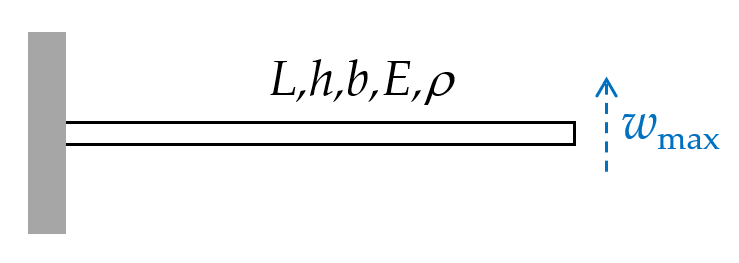
\includegraphics[width=0.72\linewidth,height=0.28\textheight,keepaspectratio]{figures/extracted-011.png}
\end{center}
\subsection{B.5 CALCULATE VIBRATION OF A PLUCKED REED}

Consider a cantilever beam of length L=14mm and cross-section dimensions h=0.3mm, b=0.75mm. The material is steel with E=200GPa and ρ=7850 kg/m3. The beam is plucked with an initial tip displacement wmax=0.15mm. The purpose is to calculate the response w(x,t) of the plucked beam using the modal expansion method. Recall the appropriate results from class and/or BB notes and do the following:\par
\hangindent=2em\noindent\textbf{(1)} Display input data\par
\hangindent=2em\noindent\textbf{(2)} Calculate cross-section area A, mass per unit length m, cross-\par
section second moment of area I, flexural stiffness EI, and flexural constant a\par
\hangindent=2em\noindent\textbf{(3)} Calculate the roots of the cantilever eigenvalue equation for\par
j=1,...,N with N=5\par
\hangindent=2em\noindent\textbf{(4)} Calculate the fundamental Hz frequency f1 and state the symbol\par
(letter and octave) of the nearest musical note. Calculate the fundamental mode period τ1\par
\hangindent=2em\noindent\textbf{(5)} Recall the formulas for cantilever beam modeshapes and plot the\par
modes j=1,...,N\par
\hangindent=2em\noindent\textbf{(6)} calculate and plot the initial deformed shape of the beam w0(x)\par
\hangindent=2em\noindent\textbf{(7)} Assume the modal expansion method, calculate the modal\par
coefficients Aj, j=1,...,N, and do a bar plot\par
\hangindent=2em\noindent\textbf{(8)} plot the time response of the tip of the beam w(L,t) for three\par
fundamental-mode periods\par
\hangindent=2em\noindent\textbf{(9)} Comment on your results\par
\section{Extra Credit Challenge Problems}
Challenge problems are optional.\par
\subsection{C.1 ANALYZE FLEXURAL VIBRATION IN A FREE-FREE BEAM}
\hangindent=2em\noindent\textbf{(1)} sketch a free-free beam indicating all the information needed for\par
the analysis\par
\hangindent=2em\noindent\textbf{(2)} write the boundary conditions at the two ends of the beam in\par
terms of displacement w(x,t) and stress resultants M(x,t), V(x,t)\par
\hangindent=2em\noindent\textbf{(3)} repeat all the steps of Section B.2\par
\begin{center}
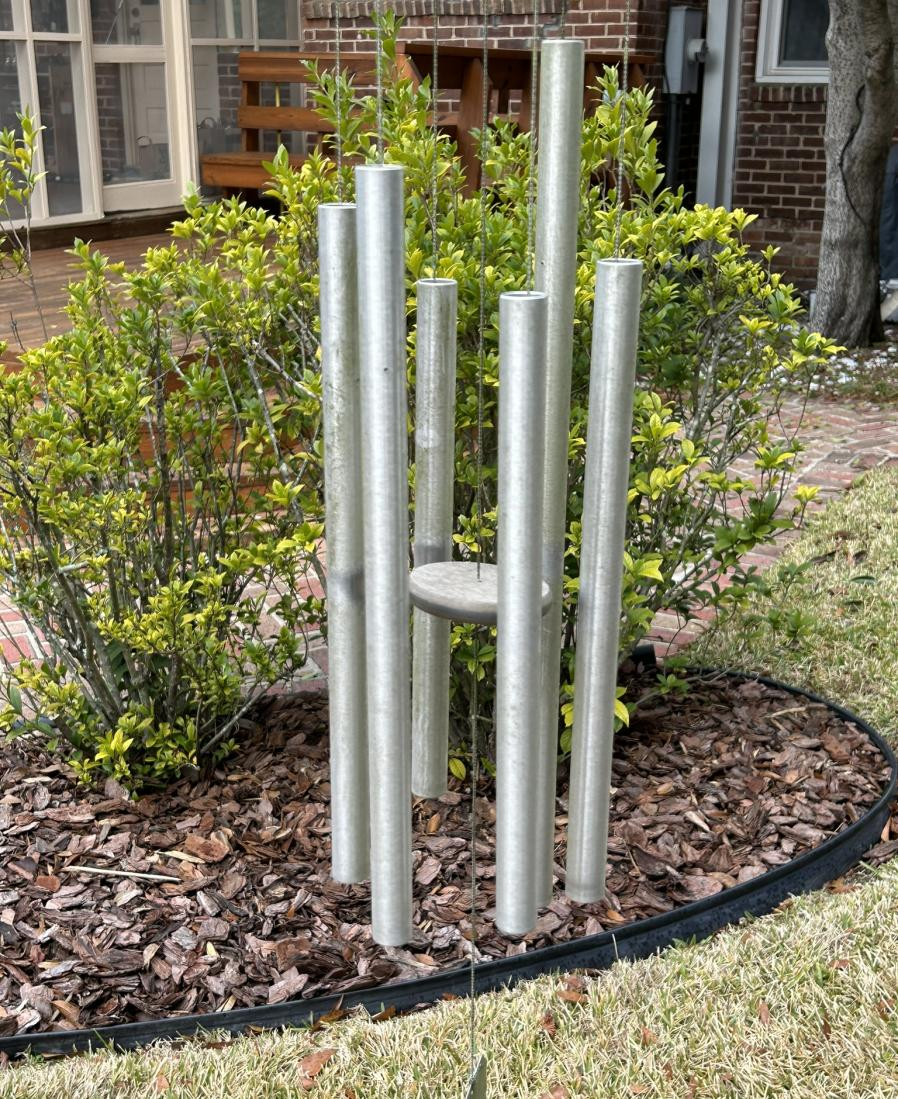
\includegraphics[width=0.72\linewidth,height=0.28\textheight,keepaspectratio]{figures/extracted-012.png}
\end{center}
\subsection{C.2 CALCULATE WIND-CHIME TONES}
Consider the wind chime shown in Figure 8 and Figure 9.\par

\begin{center}\small\itshape Figure 8 Wind chime\end{center}
\begin{center}

\includegraphics[width=0.72\linewidth,height=0.28\textheight,keepaspectratio]{figures/extracted-013.png}
\end{center}
\begin{center}\small\itshape Figure 9 Tubes of the wind chime with the suspension points circled in\end{center}
red.\par

The wind chime tubes are made of aluminum with E=70GPa and ρ=2700kg/m3. The outer and inner diameters of the tubes are D=22.3 mm; d=19.4 mm. The tube length is L. Each tube is suspended at a distance e from its end. The L and e values are given in Table 2.\par

\begin{center}\small\itshape Table 2: The measured L and e values of the six wind chime tubes\end{center}
\# L, mm e, mm 1 500 110 2 352 78 3 312 70 4 332 74 5 384 87 6 406 90\par

Use the free-free beam analysis developed in Problem C.1 to perform the engineering evaluation of the wind chime tubes. Do the following:\par
\hangindent=2em\noindent\textbf{(1)} calculate the cross-section area A\par
\hangindent=2em\noindent\textbf{(2)} calculate mass per unit length m\par
\hangindent=2em\noindent\textbf{(3)} calculate second moment of area I\par
\hangindent=2em\noindent\textbf{(4)} calculate flexural stiffness EI\par
\hangindent=2em\noindent\textbf{(5)} calculate flexural constant a\par
\hangindent=2em\noindent\textbf{(6)} use the MATLAB function fzero to find the first root of the\par
transcendental eigenvalue equation defined in Problem C.1\par
\hangindent=2em\noindent\textbf{(7)} use the length values given in Table 2 to calculate the\par
wavenumber γ and the corresponding frequencies ω1 and f1 for each of the six tubes\par
\hangindent=2em\noindent\textbf{(8)} use https://www.phys.unsw.edu.au/music/note/ to estimate the\par
musical notes that might be associated with the frequencies of the six tubes\par
\hangindent=2em\noindent\textbf{(9)} Graduate work:\par
\hangindent=2em\noindent\textbf{(a)} calculate and plot the modeshape W1(x) for each of the six\par
tubes\par
\hangindent=2em\noindent\textbf{(b)} estimate the location x0 where the modeshape W1(x) crosses\par
the zero line, compare the values x0 with the values e given in Table 2, and calculate percentage difference. Comment on your results\par
\hangindent=2em\noindent\textbf{(10)} Graduate work: find by manual iterations the adjusted tube\par
length values that will give exact musical notes without \# at item (8) above\par
\subsection{C.3 CALCULATE FLEXURAL VIBRATION IN A FREE-FREE BEAM}
Assume a free-free beam of length L=445 mm, and cross-section dimensions h=3mm, b=37mm. The material is steel with E=200GPa and ρ=7850 kg/m3. Do the following:\par

Repeat the steps of Section B.3\par
\subsection{C.4 ANALYZE FLEXURAL VIBRATION OF SIMPLY SUPPORTED}
BEAM\par
\hangindent=2em\noindent\textbf{(1)} sketch a simply supported beam indicating all the information\par
needed for the analysis\par
\hangindent=2em\noindent\textbf{(2)} write the boundary conditions at the two ends of the beam in\par
terms of displacement w(x,t) and stress resultants M(x,t), V(x,t)\par
\hangindent=2em\noindent\textbf{(3)} recall from class notes the general solution w(x,t) consisting of\par
the multiplication of two terms:\par
\hangindent=2em\noindent\textbf{(a)} first term: a function W(x) depending on constants C1, C2,\par
C3, C4, and trigonometric and hyperbolic functions of γx\par
\hangindent=2em\noindent\textbf{(b)} second term: a complex exponential function of ωt\par
\hangindent=2em\noindent\textbf{(4)} substitute (3) into (2) and write boundary conditions in terms\par
of constants C1, C2, C3, C4\par
\hangindent=2em\noindent\textbf{(5)} solve (4) for C2, C4 and obtain a set of equations for C1, C3\par
\hangindent=2em\noindent\textbf{(6)} discuss the trivial solution\par
\hangindent=2em\noindent\textbf{(7)} choose to search for the nontrivial solution and define the\par
equation that needs to be solved to find a nontrivial solution\par
\hangindent=2em\noindent\textbf{(8)} introduce the notation z=γL and write the eigenvalue equation\par
in terms of z\par
\hangindent=2em\noindent\textbf{(9)} write the general expression of the roots zj of the eigenvalue\par
equation\par
\hangindent=2em\noindent\textbf{(10)} use item (8) to write the general expression for the\par
wavenumber γj in terms of j and length L\par
\hangindent=2em\noindent\textbf{(11)} Recall from class notes the definition of wavenumber γ in\par
terms of frequency ω and flexural constant a\par
\hangindent=2em\noindent\textbf{(12)} solve (11) for frequency ω in terms of wavenumber γ and\par
flexural constant a\par
\hangindent=2em\noindent\textbf{(13)} use (10) and (12) to write the general expression of the natural\par
frequency ωj in terms of j, beam constant a, and beam length L\par
\hangindent=2em\noindent\textbf{(14)} recall definition of a in terms of bending stiffness EI and mass\par
per unit length m and obtain an expression for the natural frequencies ωj and fj in terms of j, EI, m, L\par
\hangindent=2em\noindent\textbf{(15)} use item (5) to solve for C3\par
\hangindent=2em\noindent\textbf{(16)} substitute the values found so far for C2, C3, C4 and write W(x)\par
in terms of C1 and γx\par
\hangindent=2em\noindent\textbf{(17)} Set C1=1 and write the modeshapes Wj(x) in terms of γj\par
\hangindent=2em\noindent\textbf{(18)} give the expression of modeshape orthonormality\par
\subsection{C.5 CALCULATE SIMPLY SUPPORTED FLEXURAL VIBRATION}
Assume a simply supported beam of length L=445 mm, and cross- section dimensions h=3mm, b=37mm. The material is steel with E=200GPa and ρ=7850 kg/m3. Do the following: Repeat the steps of Section B.3\par
\begin{center}

\includegraphics[width=0.72\linewidth,height=0.28\textheight,keepaspectratio]{figures/extracted-014.png}
\end{center}
\subsection{C.6 ANALYSIS OF WAVE EQUATION IN A SLENDER BAR}
Assume a uniform slender bar of cross section A and density ρ (Figure 10). The bar undergoes time-varying axial displacement u(x,t). The displacement is assumed uniform across the bar cross section.\par

\begin{center}\small\itshape Figure 10 Wave motion in a uniform slender bar\end{center}

Do the following:\par
\hangindent=2em\noindent\textbf{(1)} state the assumption made about motion and deformation in the\par
slender bar\par
\hangindent=2em\noindent\textbf{(2)} draw free-body diagram (FBD) of an infinitesimal bar element\par
of length dx and write Newton’s law of motion (NLM) equation\par
\hangindent=2em\noindent\textbf{(3)} write elasticity equation that relates stress and displacement\par
\hangindent=2em\noindent\textbf{(4)} substitute (3) into (2) and derive the partial differential equation\par
(PDE) in terms of displacement\par
\hangindent=2em\noindent\textbf{(5)} define the wavespeed c in terms of elasticity modulus E and\par
density ρ\par
\hangindent=2em\noindent\textbf{(6)} write the wave equation\par
\hangindent=2em\noindent\textbf{(7)} assume separation of x and t variables and write the solution as\par
a product between an x function U(x) and an exponential function in t of the form e-iωt\par
\hangindent=2em\noindent\textbf{(8)} substitute (7) into (6) and derive an ordinary differential\par
equation (ODE) in terms of c, ω, U(x)\par
\hangindent=2em\noindent\textbf{(9)} recall from HW01 the definition of wavenumber γ in terms of\par
frequency ω and wavespeed c and use it to simplify (8)\par
\hangindent=2em\noindent\textbf{(10)} assume U(x) as an exponential function of x of the form esx\par
\hangindent=2em\noindent\textbf{(11)} substitute (10) into (9) and derive the characteristic equation\par
\hangindent=2em\noindent\textbf{(12)} find the roots s1, s2 of the characteristic equation in terms of the\par
wavenumber γ and write the general solution U(x) in terms of complex exponentials of γx\par
\hangindent=2em\noindent\textbf{(13)} add the time dependency defined at (7) and write the general\par
solution for u(x,t) in terms of complex exponentials of γx, ωt, and constants A1, A2\par
\hangindent=2em\noindent\textbf{(14)} rewrite the general solution (13) in terms of constants C1, C2,\par
trigonometric functions of γx and a complex exponential function of ωt\par
\hangindent=2em\noindent\textbf{(15)} Graduate Work: identify the forward and backward waves in\par
the general solution derived at (13)\par
\subsection{C.7 CALCULATE AXIAL VIBRATION WITH VARIOUS BOUNDARY}
\subsubsection*{Conditions}
Consider a slender aluminum bar of diameter D=20 mm and length L=3.0 m. Common values for aluminum elastic modulus and density are E=70 GPa and ρ=2700 kg/m3. The bar undergoes axial vibration with frequency ω. The purpose is to calculate the string vibration characteristics, the modeshapes, for j=1,...,N modes with N=5. We should also verify mode orthonormality using numerical integration on a linspace(0,L,Nx) with Nx=1000. Three boundary condition cases are considered:\par

boundary conditions case x=0 x=L\par
\hangindent=2em\noindent\textbf{(a)} fixed fixed\par
\hangindent=2em\noindent\textbf{(b)} fixed free\par
\hangindent=2em\noindent\textbf{(c)} free free\par

\hangindent=2em\noindent\textbf{(1)} Display input data\par
\hangindent=2em\noindent\textbf{(2)} Calculate wavespeed c\par
Then, for each of the three cases, do the following:\par
\hangindent=2em\noindent\textbf{(3)} Display boundary conditions\par
\hangindent=2em\noindent\textbf{(4)} Calculate and display modal vibration characteristics\par
\hangindent=2em\noindent\textbf{(5)} Calculate and plot overlapped the displacement modeshapes\par
\hangindent=2em\noindent\textbf{(6)} Verify modeshape orthonormality by numerical integration\par
\hangindent=2em\noindent\textbf{(7)} Calculate and plot overlapped the normalized stress modeshapes\par
\hangindent=2em\noindent\textbf{(8)} Discuss your results\par
\begin{center}
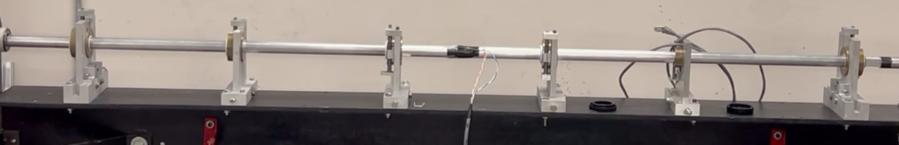
\includegraphics[width=0.72\linewidth,height=0.28\textheight,keepaspectratio]{figures/extracted-015.png}
\end{center}
\subsection{C.8 CALCULATE THE HOPKINSON BAR}

https://en.wikipedia.org/wiki/Split-Hopkinson\_pressure\_bar\par

The Hopkinson pressure bar is used to create and measure axial stress pulses. It consists of a long and slender metallic bar which is hit at one end. The hit creates a stress pulse that propagates in the bar and is measured by strain gauges. A common application is to measure the compression behavior of a small specimen placed in what is called the Split-Hopkinson bar. Consider an aluminum Hopkinson pressure bar of diameter D=20mm. Common values for aluminum elastic modulus and density are E=70GPa and ρ=2700kg/m3. Do the following:\par
\hangindent=2em\noindent\textbf{(1)} Calculate the axial wavespeed c in aluminum\par
\hangindent=2em\noindent\textbf{(2)} Assume the bar length is L=3.2 m and calculate the time t\par
required to travel the length of the bar\par
\hangindent=2em\noindent\textbf{(3)} Calculate the natural frequencies f1, f2, f3 of the first three\par
modes of bar axial vibration\par
\hangindent=2em\noindent\textbf{(4)} Calculate and plot the corresponding axial vibration\par
modeshapes\par
\hangindent=2em\noindent\textbf{(5)} Graduate Work: Research the topic of the split Hopkinson\par
pressure bar and write a short description of this apparatus and its uses\par
\begin{center}
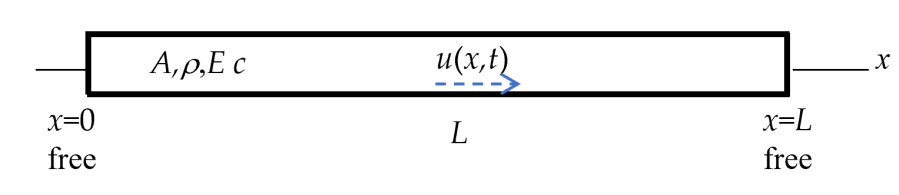
\includegraphics[width=0.72\linewidth,height=0.28\textheight,keepaspectratio]{figures/extracted-016.png}
\end{center}
\subsection{C.9 ANALYZE AXIAL VIBRATION IN A FREE-FREE BAR}
Consider a slender bar of finite length L as shown in Figure 11. The bar has cross-section area A, density ρ, elastic modulus E. The bar is free at both ends.\par

\begin{center}\small\itshape Figure 11 Vibration of a slender bar of finite length L free at both ends\end{center}

Do the following:\par
\hangindent=2em\noindent\textbf{(1)} write the boundary conditions at the two ends of the bar\par
\hangindent=2em\noindent\textbf{(2)} recall from Problem C.6 the general solution u(x,t) in terms of:\par
\hangindent=2em\noindent\textbf{(a)} first term: a function U(x) depending on constants C1, C2\par
and trigonometric functions of γx\par
\hangindent=2em\noindent\textbf{(b)} second term: a complex exponential function of ωt\par
\hangindent=2em\noindent\textbf{(3)} substitute (2) into (1) and write boundary conditions in terms\par
of constants C1, C2\par
\hangindent=2em\noindent\textbf{(4)} solve (3) for C1 and obtain an equation for C2\par
\hangindent=2em\noindent\textbf{(5)} discuss the trivial solution\par
\hangindent=2em\noindent\textbf{(6)} choose to search for a nontrivial solution and define the\par
equation that needs to be solved to find a nontrivial solution\par
\hangindent=2em\noindent\textbf{(7)} introduce the notation z=γL and write the eigenvalue equation\par
in terms of z\par
\hangindent=2em\noindent\textbf{(8)} solve the eigenvalue equation and write the general expression\par
for the eigenvalues zj , j=1,2,3,...\par
\hangindent=2em\noindent\textbf{(9)} use (8) to write the general expression for the wavenumber γj\par
in terms of j and length L\par
\hangindent=2em\noindent\textbf{(10)} Recall from HW01 the definition of wavenumber γ in terms of\par
frequency ω and wavespeed c\par
\hangindent=2em\noindent\textbf{(11)} use (10) to solve for frequency ω in terms of wavenumber γ\par
and wavespeed c\par
\hangindent=2em\noindent\textbf{(12)} use (9) and (11) to write the general expression of the natural\par
frequency ωj in terms of j, wavespeed c, and bar length L\par
\hangindent=2em\noindent\textbf{(13)} use (12) to write the general expression of the Hz frequency fj\par
in terms of j, wavespeed c, and length L\par
\hangindent=2em\noindent\textbf{(14)} explain the meaning of fundamental frequency and overtones\par
\hangindent=2em\noindent\textbf{(15)} recall from HW01 the relationship between wavelength λ and\par
wavenumber γ\par
\hangindent=2em\noindent\textbf{(16)} use (9) into (15) to write the general expression for the\par
wavelength λj in terms of j and length L\par
\hangindent=2em\noindent\textbf{(17)} use (16) to explain which wavelength multiples could be\par
accommodated vibratory standing waves in a bar of length L fixed at both ends\par
\hangindent=2em\noindent\textbf{(18)} recall U(x) from (2)(a) and use (4) to eliminate C1\par
\hangindent=2em\noindent\textbf{(19)} set C2=1 and write the general expression of the modeshape\par
Uj(x) in terms of the wavenumber γj\par
\hangindent=2em\noindent\textbf{(20)} give the expression of modeshape orthonormality\par
\hangindent=2em\noindent\textbf{(21)} write the general expression of the stress modeshapes\par
\subsection{C.10 ANALYZE AXIAL VIBRATION IN A FIXED-FIXED BAR}
Do the following:\par
\hangindent=2em\noindent\textbf{(1)} sketch a bar fixed at both ends indicating all the information\par
needed for the analysis\par
\hangindent=2em\noindent\textbf{(2)} write the boundary conditions at the two ends of the bar\par
\hangindent=2em\noindent\textbf{(3)} repeat the steps of Problem C.9\par
\subsection{C.11 ANALYZE AXIAL VIBRATION IN A FIXED-FREE BAR}
Do the following:\par
\hangindent=2em\noindent\textbf{(1)} sketch a bar fixed at one end and free at the other end indicating\par
all the information needed for the analysis\par
\hangindent=2em\noindent\textbf{(2)} write the boundary conditions at the two ends of the bar\par
\hangindent=2em\noindent\textbf{(3)} repeat the steps of Problem C.9\par
\end{document}
